
%
% Einlesen der .sty-Dateien
%
%  se-pa1-input-styles.tex
%
%  Joerg Baumgart 01.08.2011
%
%  Zusammenfassung und Konfiguration wichtiger Styles f\"ur die 
%  Erzeugung von Seminar-, Projekt- und Bachelorarbeiten
%
%  2012-03-12: auf Version 0.94 umgestellt
%
%
\documentclass[12pt,BCOR=10mm,headinclude=on,footinclude=off,bibliography=totoc]{scrreprt}
\usepackage[T1]{fontenc}
\usepackage[utf8]{inputenc}
\usepackage[ngerman]{babel} % Deutsche Einstellungen
\usepackage{lmodern}

\usepackage{tikz} % Graphikpaket, das zu pdfLaTeX kompatibel ist
\usepackage{xkeyval} % Definition von Kommandos mit mehreren optionalen Argumenten
\usepackage{listings} % Formatierung von Programmlistings
\usepackage{graphicx} % Einbinden von Graphiken
\usepackage{ifthen}
\usepackage{color}
\usepackage{slashbox} % Diagonalen in Tabellenfeldern
\usepackage{framed} % Erzeugung schwarzer Linien am linken Rand zur Hervorhebung von Textteilen
\usepackage{caption} % Korrektes Setzen einer mehrzeiligen float-Unterschrift bei neu definierten float-Umgebungen
\usepackage{floatrow}

% Es wird jeweils die sty-Datei importiert und entsprechende Konfigurationseinstellungen werden vorgenommen

\usepackage{se-jb-scrpage2} % Formatierung der Kopf- und Fu{\ss}zeilen
\usepackage{se-jb-footmisc}    % Fussnoten besser formatieren

\usepackage{se-jb-glossaries-v094} % Abk\"urzungsverzeichnis, Symbolverzeichnis, Glossar
   
\usepackage{se-jb-floatrow}    % Definition und Konfiguration von float-Umgebungen (figure, table, die neue programm-Umgebung)
% Achtung: se-jb-varioref muss nach se-jb-floatrow importiert werden; 
% andernfalls ist der counter programm f\"ur die labelformat-Anweisung noch nicht definiert   
\usepackage{se-jb-varioref}   % Definition von Querverweisen
\usepackage{se-jb-chngcntr}   % Kapitelweise oder globale Nummerierung von Abbildungen etc.
   
\usepackage{se-jb-listen} % Definition neuer, besser formatierter Listen
%\usepackage{pdf-kommandos} 
\usepackage{se-jb-kommandos-v094} % neue Kommandos f\"ur Seminar-, Projekt- und Bachelorarbeiten


\usepackage{tabulary}
\usepackage{eurosym}

%
% Individuelle Konfiguration des Dokumentes
%
%  Individuelle Konfiguration einer Projektarbeit
%
%
%
%

%
% Literaturverzeichnis
% 
\usepackage{se-jb-jurabib-theisen} % Literaturverzeichnis gem\"ass den Vorgaben von Theisen aufbauen



% Weitere Optionseinstellungen f\"ur das Koma-Script
%
% Zwischen Abs\"atzen einen Abstand von 0.5 \baselineskip erzeugen
\KOMAoption{parskip}{full}
%
% Vergleiche Duden "Gliederung von Nummern, S.111" 
% DIN 5008 anschauen, wenn sie neu ver\"offentlicht wurde
\KOMAoption{numbers}{noendperiod}
%
%



%  Voreinstellungen f\"ur floats
%  Durch die verwendeten Parameter wird die Wahrscheinlichkeit deutlich kleiner, 
%  dass Gleitobjekte (z. B. Abbildungen) ans Ende des Dokumentes verschoben 
%  werden; 
%  Achtung: clearpage erzwingt die Ausgabe von Gleitobjekten
%
\renewcommand{\topfraction}{1}  % Gleitobjekte d\"urfen eine Seite zu 100% belegen 
\renewcommand{\bottomfraction}{1} % Entsprechender Wert f\"ur den unteren Teil der Seite
\renewcommand{\textfraction}{0} % Eine Seite darf auch ohne Fliesstext existieren
%%%\renewcommand{\floatpagefraction}{1} % Bedeutung unklar, daher keine Ver\"anderung des Vorgabewertes 
                                                                        % von 0.5; eventuell bringt ein \"Anderung auf 1 etwas, wenn 
                                                                         % Probleme mit floats auftreten
                                                                         
                                                                         
                                                                         
% Konfiguration von Programm-Listings
% 
% Achtung: hier gibt es nahezu beliebig viele weitere Konfigurationm\"oglichkeiten; vgl. Paketdokumentation
%
%\lstset{
%	language=Java,
%	basicstyle=\ttfamily,
%	keywordstyle=\color{blue},
%	captionpos=b,
%	aboveskip=0mm,
%	belowskip=0mm,
%   xleftmargin=0em
%}

\lstdefinelanguage{JavaScript} {
	morekeywords={
		break,const,continue,delete,do,while,export,for,in,function,
		if,else,import,in,instanceOf,label,let,new,return,switch,this,
		throw,try,catch,typeof,var,void,with,yield
	},
	sensitive=false,
	morecomment=[l]{//},
	morecomment=[s]{/*}{*/},
	morestring=[b]",
	morestring=[d]'
}

\lstset{
	language=JavaScript,
	basicstyle=\ttfamily,
	showstringspaces=false,
	breaklines=true,
	keywordstyle=\ttfamily\bfseries\color{RoyalBlue},
	identifierstyle=\ttfamily,
	stringstyle=\ttfamily\color{BrickRed},
	commentstyle=\color{OliveGreen},
	xleftmargin=0mm,
	xrightmargin=0mm,
	aboveskip=1em,
	belowskip=0mm
}
          
%
% Grundkonfiguration der Abs\"ande zwischen den Items der maximal f\"unf Verschachtelungsebenen der 
% neuen Listenumgebungen
%                                                                             
% Initialisierung der Abst\"ande zwischen den items f\"ur seList; Grundeinheit: 0.5\baselineskip; siehe se-jb-listen
\seSetlistbaselineskip{1}{0.75}{0.75}{0.75}{0.75}
% Initialisierung der Abst\"ande zwischen den items f\"ur seToplist; Grundeinheit: 0.5\baselineskip; siehe se-jb-listen
\seSettoplistbaselineskip{1}{0.75}{0.75}{0.75}{0.75}     


%
%  Konfiguration der verschiedenen Verzeichnisse
%
%  abstandEintrag: Wert wird mit \baselineskip multipliziert
%

%
%  Abbildungsverzeichnis
%
\seKonfigurationAbb[
%verzeichnisname=Abbildungsverzeichnis,
labeltextLinks=, % kein Text links;
%labeltextRechts=:,
labelbreite=1cm,
%labeleinzug=1cm,
%abstandEintrag=1,
%newpage=ja,
%pnumwidth=20mm,
%dotsep=1000,
%tocrmarg=4.5cm,
%abstandVerzeichnis=-1mm
]

%
% LIstingverzeichnis
%
\seKonfigurationPrg[
%verzeichnisname=Listing-Verzeichnis,
labeltextLinks=,
%labeltextRechts=:,
labelbreite=1cm,
%labeleinzug=2cm,
%abstandEintrag=1,
%newpage=ja,
%%pnumwidth=20mm,
%dotsep=1000,
%tocrmarg=4.5cm,
%abstandVerzeichnis=-10mm
]

%
% Tabellenverzeichnis
%
\seKonfigurationTab[
%verzeichnisname=Liste der Tabellen,
labeltextLinks=,
%labeltextRechts=:,
labelbreite=1cm,
%labeleinzug=0.5cm,
%abstandEintrag=1,
%newpage=ja,
%pnumwidth=20mm,
%dotsep=1000,
%tocrmarg=4.5cm,
%abstandVerzeichnis=-10mm
]

%
% Abk\"urzungsverzeichnis
%
\seKonfigurationAbk[
%verzeichnisname=Liste der Abk\"urzungen,
%labelbreite=3cm,
%labeleinzug=0.5cm,
%abstandEintrag=1,
%newpage=ja,
%abstandVerzeichnis=-10mm
]

%
% Symbolverzeichnis
% 
\seKonfigurationSym[
%verzeichnisname=Liste der Symbole,
%labelbreite=4cm,
%labeleinzug=3.5cm,
%abstandEintrag=1,
%newpage=ja,
%abstandVerzeichnis=-10mm
]

%
% Glossar
%
\seKonfigurationGlo[
%verzeichnisname=Glossar,
%abstandEintrag=0,
]



% (eventuelle) Neudefinition f\"ur die Unter-/\"Uberschriften von Abbildungen, Tabellen und Listings
%
%
%\renewcommand{\seCaptionNameAbbildung}{Abb.}
%\renewcommand{\seCaptionNameTabelle}{Tab.}
%\renewcommand{\seCaptionNameProgramm}{Prg.}


% % (eventuelle) Neudefinition f\"ur Querverweise innerhalb des Textes
%
%
%
%\renewcommand{\seQuerverweisSeite}{Seite}
%\renewcommand{\seQuerverweisAbbildung}{Abb.}
%\renewcommand{\seQuerverweisTabelle}{Tab.}
%\renewcommand{\seQuerverweisProgramm}{Prg.}
%\renewcommand{\seQuerverweisKapitel}{Kap.}
%\renewcommand{\seQuerverweisGleichung}{Gl.}

% Kommandos, die direkt nach \begin{document} ausgef\"uhrt werden m\"ussen
%
%
%
\AtBeginDocument{%
\renewcommand{\listfigurename}{\seAbbildungenVerzeichnisname}
\renewcommand{\listtablename}{\seTabellenVerzeichnisname}
\renewcommand{\figurename}{\seCaptionNameAbbildung}
\renewcommand{\tablename}{\seCaptionNameTabelle}
\pagenumbering{roman}
}
                                                              
                                                                         

%
% Definition von Abk\"urzungen, Symbolen und eventuell Glossareintr\"agen
%
% 2012-03-22 Verwendung des optionalen Parameters f\"ur die Pluralform einer Abk\"urzung
%
% 2012-02-06 Umstellung auf die neuen Kommandos
%
%
%
%  J\"org Baumgart
%  Definition einiger Abk\"urzungen
%  


% Definition von Abk\"urzungen
%
% 1. Parameter: Schluessel (key) der Abkuerzung
% 2. Parameter: Abkuerzung
% 3. Parameter: Vollform
% 4. Parameter: Vollform im Plural (optional; falls nicht definiert, wird der Wert des dritten Parameters verwendet)
%
\seNewAcronymEntry{sdk}{SDK}{Software Development Kit}{Software Development Kits}

% 2012-03-24
% \"Uber den optionalen Parameter in eckigen Klammern wird die Pluralform f\"ur das erste 
% Auftreten der Abk\"urzung definiert

\seNewAcronymEntry[URLs]{url}{URL}{Uniform Resource Locator}%
{Uniform Resource Locators}






% Alternative Definition von Abk\"urzungen; diese sollten nicht verwendet werden!!!
%
%\newacronym{dhbw}{DHBW}{Duale Hochschule Baden-W\"urttemberg}
%\newacronym{usb}{USB}{Universal Serial Bus}


% Alternative Definition von Symbolen
%
% Achtung: ohne sort wird nach Name sortiert
%\newglossaryentry{pi}{
%name=$\pi$,
%description={Die Kreiszahl},
%type=symbolslist,
%sort=b
%}
%
%\newglossaryentry{ND}{
%name=$\mbox{\textsl{ND}}$,
%description={Nutzungsdauer einer Maschine},
%type=symbolslist,%
%sort=a
%}



% Alternative Definition von Glossareintr\"agen
%
%\newglossaryentry{glos:AD}{
%first=Active Directory\textsuperscript{GL},
%name=Active Directory,
%description={Active Directory ist in einem Windows 2000/Windows
%Server 2003-Netzwerk der Verzeichnisdienst, der die zentrale
%Organisation und Verwaltung aller Netzwerkressourcen erlaubt. Es
%erm\"oglicht den Benutzern \"uber eine einzige zentrale Anmeldung den
%Zugriff auf alle Ressourcen und den Administratoren die zentral
%organisierte Verwaltung, transparent von der Netzwerktopologie und
%den eingesetzten Netzwerkprotokollen. Das daf\"ur ben\"otigte
%Betriebssystem ist entweder Windows 2000 Server oder
%Windows Server 2003, welches auf dem zentralen
%Dom\"anencontroller installiert wird. Dieser h\"alt alle Daten des
%Active Directory vor, wie z.\,B. Benutzernamen und
%Kennw\"orter.\protect\seFootcite{Vgl.}{S. 200}{Dud09}}
%}














 

%\seIstErsteProjektarbeit{}
\seIstZweiteProjektarbeit{}
%\seIstBachelorarbeit{}

\newcommand{\version}{0.95}

% 
% Diese Redefinition ist nur f\"ur den Anhang B der  
% Vorlage (Hinweise zur Installation und \"Ubersetzung)
% notwendig; f\"ur Ihre Projekt-/Bachelorarbeit spielt sie keine Rolle
%
\renewcommand{\seVorlage}{\jobname}


\begin{document}

% Erzeugung des Titelblatts
%
%
%
\seTitelblattWissenschaftlicheArbeit[
%hilfslinien=ja,
%dhbwlogoSkalierung=0.5,
%dhbwlogoDeltaX=2.4,
%dhbwlogoDeltaY=-10,
firmenlogo=firmenlogo,
firmenlogoSkalierung=0.5,
firmenlogoDeltaX=0,
firmenlogoDeltaY=0,
studiengang=\seWirtschaftsinformatik,
studienrichtung=\seSoftwareEngineering,
thema=\seThemaWaArbeit{},
verfasser=Mike Mülhaupt,
%verfasserin=,
matrikelnummer=1366418,
kurs=WWI\,11\,SE\,B,
firma=ALDI Einkauf GmbH \& Co. oHG,
% Da im Text ein Komma enthalten ist, muss der Text eingeklammert werden
abteilung=IIT Stores,
%studiengangsleiterin=,
studiengangsleiter=Prof. Dr.-Ing. J\"org Baumgart,
%wissenschaftlicheBetreuerinName=Dr. Melanie Mustermann,
%wissenschaftlicheBetreuerinEmail=melanie.mustermann@musterfirma.de,
%wissenschaftlicheBetreuerinTelefon=0621/999999,
wissenschaftlicherBetreuerName=Prof. Dr.-Ing. J\"org Baumgart,
wissenschaftlicherBetreuerEmail=joerg.baumgart@dhbw-mannheim.de,
wissenschaftlicherBetreuerTelefon=+49\,(0)624\,4105\,-\,1216,
firmenbetreuerinName=Ulrike Gasch,
firmenbetreuerinEmail=ulrike.gasch@aldi-sued.com,
firmenbetreuerinTelefon=+49\,(0)208\,9927 - 1818,
%firmenbetreuerName=,
%firmenbetreuerEmail=,
%firmenbetreuerTelefon=,
bearbeitungszeitraumVon=29. Juli 2013,
bearbeitungszeitraumBis=11. November 2013,
% ja/nein
sperrvermerk=ja
]





% Erzeugung der Kurzfassung; Verfasser, Firma und Thema werden automatisch \"ubernommen
%
% Der optionale Parameter kann verwendet werden, um f\"ur das Thema der Arbeit eine 
% andere Formatierung vorzunehmen; das sollte in der Regel nicht erforderlich sein;
% ausserdem besteht die Gefahr inkonsistenter Titel auf dem Titelblatt und in der 
% Kurzfassung
%
%\seKurzfassung{} % dieses Kommando sollte standardm\"assig verwendet werden

\seKurzfassung[]


% Beispiel f\"ur ein Kapitel, dass vor dem Einleitungskapitel kommt, z. B. ein Vorwort oder eine Danksagung
%\seKapitelVorEinleitung{Vorwort}

%Muss jetzt wirklich nicht sein, aber wenn Sie unbedingt (z. B.) Ihrem Haustier f\"ur die Unterst\"utzung bei 
%der Anfertigung der Projektarbeit danken wollen ...; vgl. auch das Dokument \textsl{Empfehlungen und 
%Hinweise zur Anfertigung der ersten Projektarbeit}

% 2012-02-06 Inhaltsverzeichnis muss vor den weiteren Verzeichnisses kommen
%
%
% Ausgabe des Inhaltsverzeichnisses
%
%
\seInhaltsverzeichnis[%
einrueckung=ja,
gliederungsebenen=4
]




% Ausgabe der verschiedenen Verzeichnisse
% abk: Abk\"urzungsverzeichnis
% sym: Symbolverzeichnis
% abb: Abbildungsverzeichnis
% tab: Tabellenverzeichnis
% prg: Listingverzeichnis
%
%
% Achtung: Abk\"urzungs- und Symbolverzeichnis werden nur ausgegeben, wenn mindest ein Symbol bzw. 
%                mindestens eine Abk\"urzung in der Arbeit verwendet wurden
%
%
% gliederungsebene:
% -- section: die Verzeichnisse werden einem Kapitel "Verzeichnisse" untergliedert
% -- chapter: die Verzeichnisse sind jeweils eigene Kapitel
% imInhaltsverzeichnis: ja/nein -- Sollen die Verzeichnisse im Inhaltsverzeichnis enthalten sein?
\seVerzeichnisse[gliederungsebene=section,imInhaltsverzeichnis=ja]{abk}{sym}{abb}{tab}{prg}






% Erstes eigentliches Kapitel der Arbeit; typischerweise das Einleitungskapitel;
% hier muss wieder auf die Nummierung mit arabischen Seitenzahlen umgestellt werden
%
\chapter{Einleitung}\pagenumbering{arabic}
Der Kunde, der seinen Wocheneinkauf in einem gewöhnlichen Supermarkt erledigt, muss alle Artikel, die er kaufen möchte, zunächst aus dem Regal in seinen Einkaufswagen, anschließend von dort auf das Kassenband und ein letztes Mal vom Kassentisch zurück in den Einkaufswagen legen. D.h. jeder Artikel muss drei Mal in die Hand genommen werden, bis er sich schließlich im Besitz des Kunden befindet. Welchen Aufwand dies mit sich bringt, ist jedoch nur den Kunden bewusst, die einen vollgeladenen Einkaufswagen zur Kasse schieben.

Um diesen Aufwand zu vermeiden, wurde in der ersten Projektarbeit ein Konzept erarbeitet, womit der Kunde seine Artikel selbstständig erfassen kann und anschließend nur noch bezahlen muss. Die quantitativen Vorteile, die ein solches System mit sich bringt, lassen sich ohne praktische Erfahrung allerdings schwer einschätzen. Daher soll im Rahmen dieser Arbeit ein Proof of Concept realisiert werden, mit dessen Hilfe der Prozess des mobilen SelfScannings praktisch erfahren, getestet und bewertet werden kann.

\section{Zielsetzung}
Ein fachliches Lösungskonzept für den Einsatz eines mobilen SelfScanning-Systems bei ALDI SÜD wurde in der ersten Projektarbeit bereits erarbeitet und dokumentiert. Darüber hinaus wurden die daraus resultierenden Anforderungen an die mobile Applikation identifiziert und eine mögliche Benutzerführung der App in Form eines Mock-Ups dargestellt.

Ziel dieser Arbeit ist, den Prozess im Sinne der Softwareentwicklung fortzusetzen, d.h. die mobile Applikation als Prototypen zu entwerfen und zu implementieren. Zur Ergänzung des fachlichen Konzepts sollen ferner mögliche „mobile Payment“ Lösungen identifiziert und bewertet werden.

\section{Methodische Vorgehensweise}
Die Marktanalyse soll lediglich durch Recherche bestehender Literatur, nicht durch Erhebung neuer empirischer Daten, erfolgen. Sie umfasst eine Abschätzung des derzeitigen Marktvolumens und der zukünftigen –entwicklung, sowie eine mögliche Marktstrukturierung nach Produktgruppen. Anschließend sollen einzelne Payment-Lösungen näher erläutert werden und eingeordnet werden. Zur Recherche werden neben der in Bibliotheken vorhandenen Literatur auch Statistiken von Zahlungsinstituten oder Marktforschungsunternehmen zum Einsatz kommen.

Zur Entwicklung der mobilen Applikation werden zunächst die grundsätzlichen Herangehensweisen ermittelt und anhand von fachlichen und technischen Anforderungen an das Projekt bewertet. Da die zur Verfügung stehenden Konzepte der App-Entwicklung aufgrund fehlender Erfahrungen gänzlich unbekannt sind, soll der Entwicklungsprozess dem Evolutionären Vorgehensmodell nach [Gilb („Evolutionary development“)] erfolgen. Das bedeutet, dass zunächst nur eine Kernanforderung entworfen und unmittelbar danach implementiert wird. Erkenntnisse, die sich aus diesem Evaluationsschritt ergeben, sollen in den Entwurf der nachfolgenden Funktionen einfließen.

Sollten sich im Laufe des Projekts Anforderungen als unvollständig oder ungünstig herausstellen, so ist eine Ergänzung, Änderung oder Revidierung derselben durchaus zulässig, muss jedoch auch entsprechend dokumentiert werden.

% Erstes Hauptkapitel der Arbeit 
%
%
%
\chapter{Entwicklung mobiler Applikationen}
Die Entwicklung mobiler Applikationen lässt drei grundsätzlich verschiedene Herangehensweisen zu: die native, die webbasierte und die hybride Entwicklung. Jede Methode hat ihre Vor- und Nachteile, welche je nach Anforderungen mehr oder weniger stark gewichtet werden kann, sodass die „Best-Practice“ eine Einzelfallentscheidung darstellt.

Um die beste Herangehensweise für die Entwicklung der mobile SelfScanning-App zu ermitteln, werden in den folgenden Kapiteln zunächst die Anforderungen an die App selbst zusammengefasst und anschließend zusätzliche Anforderungen an die Entwicklungsmethode festgestellt. Davon ausgehend werden die drei Entwicklungskonzepte kurz vorgestellt und deren individuellen Vor- und Nachteile herausgestellt und gewichtet. Diese werden in einem abschließenden Fazit summiert, um die bestmögliche Entwicklungsmethode für das Projekt zu festzustellen.

\section{Ermittlung der Anforderungen}
In der ersten Projektarbeit wurden bereits Anforderungen an ein mobile SelfScanning-System bei ALDI SÜD ermittelt. Diese werden im folgenden Kapitel „Fachliche Anforderungen“ nochmals erläutert und anschließend durch die technischen Anforderungen, die sich größtenteils aus den Rahmenbedingungen des Projekts ergeben, ergänzt. Beide Anforderungsgruppen werden abschließend in einer Liste stichwortartig zusammengefasst.

\subsection{Fachliche Anforderungen}
Dem Kunden soll die Möglichkeit geboten werden, alle Artikel bereits während des Einkaufs in einer Filiale mithilfe seines Smartphones zu erfassen und in einer Liste zu speichern. Das Erfassen wird durch das Einscannen eines Barcodes auf der Artikelverpackung oder alternativ durch manuelles Suchen in einer Artikeldatenbank ermöglicht. Die Liste aller eingescannten Artikel wird bei der Bezahlung an das Kassensystem übertragen, sodass der Einkauf an einer herkömmlichen Kasse bezahlt werden kann. Das Auflegen der Artikel aufs Kassenband, anschließende Einscannen und erneute Einpacken an der Kasse entfällt somit.

Der virtuelle Warenkorb (sprich: die Liste auf dem Smartphone des Kunden, die alle Artikel enthält) soll die folgenden Einzelheiten anzeigen:

\begin{seList}
	\item Pro Artikel
	\begin{seList}
		\item EAN
		\item Artikelbezeichnung
		\item Einzelpreis
		\item Menge
		\item Gesamtpreis
		\item Mehrwertsteuersatz
		\item ggf. Pfand das zu bezahlen ist
	\end{seList}
	\item Pro Einkauf
	\begin{seList}
		\item Filiale, in welcher der Einkauf stattfindet
		\item Zeitpunkt, wann der Einkauf erstellt wurde
		\item Anzahl der Artikel im Einkaufswagen
		\item Summe brutto
		\item Summe netto
	\end{seList}
\end{seList}

Darüber hinaus gibt es folgende Anforderungen an die Artikel- und Preisinformationen, die dem Kunden angezeigt werden:
\paragraph{Vollständigkeit}
Es soll ausnahmslos jeder Artikel erfasst werden können. Hiervon nicht ausgenommen sind lose bzw. unverpackte Waren aus der O\&G-Abteilung oder dem Backautomaten, Artikel deren Preis abhängig vom Gewicht ist (sog. Gewichtsartikel), sowie Pfandbons.
Außerdem sollen auch die jeweils in der Filiale gültigen Preise angezeigt werden. Hiervon nicht ausgenommen sind Preise, die innerhalb der Filiale für einen bestimmten Zeitraum reduziert werden (z.B. Abverkauf von O\&G kurz vor Feierabend).

\paragraph{Aktualität der Daten}
Die Artikel- und insbesondere die Preisinformationen, die dem Kunden angezeigt werden, sollen stets aktuell sein. Konkret heißt das, dass der Kunde immer diejenigen Preise angezeigt bekommt, welche zum Zeitpunkt des Betretens der Filiale gültig waren. 

\paragraph{Verfügbarkeit}
Während des Einkaufs soll weder eine Verbindung zum Internet noch eine Verbindung zum Kassensystem oder dem Filialnetzwerk erforderlich sein. 

In einigen Fällen führt das Erfassen von Artikeln mithilfe des Smartphones zu Ausnahmefällen. Diese werden im Folgenden erläutert:

\begin{itemize}
	\item Um den Preis eines Gewichtsartikels bestimmen zu können, muss er zunächst gewogen werden. Da in der Filiale keine für den Kunden zugänglichen Waagen vorhanden sind, werden Gewichtsartikel nach wie vor an der Kasse gewogen. Hierfür soll, sobald sich ein Gewichtsartikel im Einkaufswagen des Kunden befinden, ein Hinweis erscheinen, mit der Bitte, den Artikel an der Kasse zum Wiegen bereitzuhalten.
	\item Ebenso soll beim Erfassen von altersbeschränkten Artikeln ein Hinweis erscheinen, dass die Volljährigkeit des Kunden an der Kasse zunächst kontrolliert werden muss.
	\item Die Bonsumme, die der Kunde auf dem Smartphone angezeigt bekommt, könnte von der Summe abweichen, die er tatsächlich zu zahlen hat. Dies könnte einer Preisveränderung während des Einkaufs oder einer internen Falschberechnung zu Schulden sein. In beiden Fällen soll die Differenz ermittelt und der Kunde darauf aufmerksam gemacht werden.
\end{itemize}

\subsection{Technische Anforderungen}
Das Einscannen eines neuen Barcodes erfordert den Zugriff auf die Kamera des Smartphones. Die Zugriffsberechtigung soll einmalig bei der Erstinstallation eingefordert werden, sodass neue Artikel schnellstmöglich hinzugefügt werden können.

Zur Synchronisation von Artikel- und Preisinformationen wird eine Internetverbindung benötigt. Die initiale Datenbereitstellung soll aufgrund der Menge lediglich per WLAN erfolgen. Die nachfolgenden, regelmäßigen Aktualisierungen können per WLAN oder mobilem Internet erfolgen. Für beide Varianten soll die Zugriffsberechtigung einmalig bei der Erstinstallation eingefordert werden, sodass Daten ohne Zustimmung des Benutzers aktualisiert werden können.

Alle Daten sollen auch dann verfügbar sein, wenn keine Verbindung zum Internet besteht. Hierfür wird Zugriff zu einem permanenten Datenspeicher benötigt, dessen Berechtigung bei der Erstinstallation eingefordert werden soll.

Eine Datenbank, welche die Daten, sowie eine Schnittstelle zur Synchronisierung der Daten bereitstellt, ist vorhanden und ist ebenso wie zusätzliche Kassenfunktionen (z.B. Wiegen von Gewichtsartikeln oder Hinweis zur Alterskontrolle) nicht Teil dieses Projektes. Lediglich beim Entwurf und Implementierung der Schnittstelle muss darauf geachtet werden, die erforderlichen Daten bereitzustellen.

Da die mobile Applikation lediglich als Prototyp implementiert werden soll, spielen Anforderungen an Performance und User-Interface zunächst eine nebensächliche Rolle. Viel wichtiger ist der Aspekt, nach kurzer Zeit erste Entwicklungsergebnisse zu erhalten und die gewonnenen Erfahrungen, gemäß dem Evolutionären Vorgehensmodell, in die nächste Iteration der Entwurfsphase einfließen zu lassen.

\subsection{Zusammenfassung}
In den vorherigen Unterkapiteln wurden die Anforderungen aus fachlicher und technischer Sich nochmals näher beschrieben. Die folgende Liste fasst diese noch einmal in Stichworten zusammen, um die Umsetzung der Anforderungen am Ende des Projekt überprüfen zu können.

\paragraph{Fachliche Anforderungen}
\begin{seList}
	\item Einkauf mithilfe des Smartphones durchführen
	\begin{seList}
		\item Einkauf eröffnen
		\item Artikel scannen / suchen
		\item Einkauf abschließen / bezahlen
	\end{seList}
	\item Verfügbarkeit von Artikel- und Preisinformationen
	\begin{seList}
		\item Aktuell -> alle gültigen Preise bis zum Zeitpunkt des Betretens der Filiale vorhanden
		\item Vollständig -> jeder Artikel soll erfasst werden können. Speziell O\&G, Gewichtsartikel, Pfandbons und Backwaren aus dem Automat
		\item Offline verfügbar -> voll funktionsfähig auch ohne WLAN und ohne mobiles Internet
	\end{seList}
	\item Einkauf soll an herkömmlicher Kasse bezahlt werden
	\item Ausnahmefälle
	\begin{seList}
		\item Gewichtsartikel -> Hinweis
		\item Altersbegrenzte Artikel -> Hinweis
		\item Summe der vom Kunden eingescannten Artikel stimmt mit tatsächlicher Summe der Artikel nicht überein -> wahrscheinlich Preisänderung während Einkauf -> „stiller Alarm“ zur Protokollierung und späterer Auswertung
	\end{seList}
\end{seList}

\paragraph{Technische Anforderungen}
\begin{seList}
	\item Uneingeschränkter Zugriff auf folgende Gerätekomponenten
	\begin{seList}
		\item Kamera (Artikelscan)
		\item Internetverbindung (Synchronisation)
		\item Datenspeicher (Datenhaltung)
	\end{seList}
	\item Artikel- und Preisdatenbank ist vorhanden und bietet Schnittstelle zur Synchronisierung mit Smartphone
	\item Schnittstelle Smartphone -> Kasse um Einkauf zu bezahlen
	\begin{seList}
		\item Kennzeichnung von Gewichtsartikeln
		\item Kennzeichnung von altersbeschränkten Artikeln
		\item Kennzeichnung der Gesamtsumme, um mit tatsächlicher Summe abzugleichen
	\end{seList}
	\item Kurze Entwicklungszeit, steile Lernkurve
\end{seList}

\section{Unterschiedliche Herangehensweisen zur App-Entwicklung}
% Mit markright kann eine verk\"urzte Version der \"Uberschrift f\"ur den Seitenkopf generiert werden
%
%
%\markright{Formaler Aufbau}
In den vorherigen Kapiteln wurden die Anforderungen an das Projekt und die mobile Applikation aufgezählt und erläutert. Davon ausgehend soll nun der geeignetste Ansatz zur Entwicklung einer App ermittelt und angewendet werden. Hierfür werden die drei Alternativen zunächst beschrieben und deren Vor- und Nachteile herausgestellt.

\subsection{Native App-Entwicklung}
Als native Apps werden eigenständige Anwendungen bezeichnet, die speziell für ein konkretes Betriebssystem implementiert werden und letztendlich nur auf diesem System installations- und lauffähig sind. Auf diese Weise können die Systemressourcen optimal ausgereizt und mithilfe entsprechender Grundkonzepte des jeweiligen Betriebssystems (Multithreading, Speicherzugriff, Grafikrendering) eine hohe Performance erzielt werden. Dieser Aspekt macht sich besonders bei komplexen Anwendungen bemerkbar. Darüber hinaus ermöglichen native Apps den Zugriff auf Gerätekomponenten, wie z.B. Kamera, GPS-Sensor oder NFC-Chip.
 
Neben den eben genannten Vorteilen auf technischer Seite, gibt es noch einen weiteren, marketingtechnischen Aspekt: native Apps werden über den offiziellen App-Store des jeweiligen Herstellers vertrieben. Potenziellen Nutzer können die App also in gewohnter Art und Weise finden, Bewertungen lesen und die App gegebenenfalls direkt auf dem Smartphone installieren. Nach der Installation befindet sich eine Verknüpfung auf dem Homescreen des Nutzers, sodass die App jederzeit verfügbar steht.

Wobei dieser Aspekt gleichzeitig auch als Nachteil zu erwähnen gilt: vor der Veröffentlichung im App-Store muss die Anwendung zunächst ein aufwendiger Freigabeprozess durchlaufen werden. Die App kann jederzeit vom Store-Betreiber abgelehnt oder nachträglich aus dem Store entfernt werden. Außerdem ist für die offizielle Entwicklung einer nativen App im Falle von Apple eine kostenpflichtige Lizenz sowie ein Mac Voraussetzung.

Hinzu kommt die aufwendige Einarbeitung für unerfahrene Entwickler. Selbst bei guter Kenntnis der zu implementierenden Sprache ist eine sorgfältige Einarbeitung in das jeweilige SDK unverzichtbar. 

\subsection{Entwicklung einer WebApp}
Eine Webanwendung wird im Gegensatz zur nativen App nicht eigenständig, sondern mithilfe eines Browsers auf dem Zielsystem ausgeführt. Sie kann durch manuelles Eingeben der URL oder Aufrufen eines Lesezeichens geöffnet werden. Im Regelfall wird keine Verknüpfung auf dem Homescreen erstellt. Eine Webanwendung unterscheidet sich also nur geringfügig von einer herkömmlichen Webseite. Die größten Unterschiede liegen in der für mobile Geräte optimierten Bedienoberfläche und dem reduzierten Funktions- und/oder Informationsumfang.

Der limitierende Faktor einer Web-App ist der jeweilige Browser, in dem die App ausgeführt wird. Funktionen, die innerhalb des Browsers nicht zur Verfügung stehen, können von der App nicht verwendet werden. So gibt es beispielsweise keine Möglichkeit, den Nutzer einer Webanwendung über anstehende Updates oder Erinnerungen per Push-Notification zu kontaktieren. 

Dank moderner Webtechnologien wie HTML5 stehen allerdings zahlreiche Möglichkeiten für den Zugriff auf Systemkomponenten zur Verfügung. Leider muss der Anwender diesen Zugriff jedes Mal explizit gewähren. Darüber hinaus ermöglicht das sog. DOM-Storage eine permanente lokale Datenspeicherung bis zu 5 bis 10MB – je nach verwendetem Browser. Die zusätzliche Integration zahlreich vorhandener JavaScript-Frameworks ermöglicht dem Entwickler auch komplexe Applikationen schnell und einfach zu entwickeln.

Eine Webanwendung muss lediglich einmal implementiert werden und ist dank der einheitlichen Webstandards auf allen Betriebssystemen lauffähig. Zur Veröffentlichung ist weder ein Freigabeprozess noch eine Lizenz notwendig. Es genügt ein Webserver auf dem die Anwendung läuft. 

\subsection{Hybride App-Entwicklung}
Hybride Apps vereinen die Eigenheiten beider Entwicklungsalternativen: sie werden mithilfe von HTML, CSS und JavaScript implementiert und anschließend in eine native App integriert. Die native App besitzt als einzige Komponente einen InApp-Browser. In diesem eingebetteten Browser wird die ursprünglich entwickelte Webanwendung gerendert.

Auf diese Weise werden die Vorteile beider Welten kombiniert: mithilfe der herkömmlichen Webtechnologien lassen sich Anwendungen relativ unkompliziert entwickeln, sind auf verschiedenen Betriebssystemen lauffähig und bieten dank der „Wrapper-App“ trotzdem den vollen Funktionsumfang einer nativen App. Für den Nutzer sind hybride Apps von nativen kaum zu unterscheiden, da sie wie gewohnt über den App-Store heruntergeladen, installiert und über ein Icon aufgerufen werden. Lediglich in den Bedienelementen lässt sich gegebenenfalls ein Unterschied zu nativen Apps erkennen.

\subsection{Fazit}
Im ersten Teil dieses Kapitels wurden nochmals die Anforderungen an die App beschrieben. Dabei wurde ersichtlich, dass besonders die Kommunikation mit externen Systemen (Artikel- und Preisdatenbank sowie Kassensystem in der Filiale), sowie die Speicherung großer Datenmengen (Offline-Verfügbarkeit aller Daten) zwei wichtige Anforderungen darstellen.

Der anschließende Vergleich der drei Herangehensweisen verdeutlichte, dass die Wahl der Entwicklungsmethode weitreichende Auswirkungen auf die Implementierung und dessen Ergebnis haben kann. So bieten native Apps selbst bei komplexen Anwendungen eine hohe Performance, der nötige Entwicklungsaufwand ist besonders für unerfahrene Entwickler jedoch äußerst hoch. Web-Apps lassen sich dagegen innerhalb kürzester Zeit mithilfe gängiger Webtechnologien entwickeln und ohne weitere Umstände (weder Lizenz noch Freigabeprozess) veröffentlichen. Dank zahlreich vorhandener Frameworks lassen sich auch komplexere Anwendungen umsetzen. Der Funktionsumfang des Browsers begrenzt den Funktionsumfang jedoch deutlich, sodass eine Web-App für dieses Projekt nicht in Frage kommt (lediglich 5-10MB Datenspeicher, keine Echtzeit-Updates über Push-Notifications). Die hybride Variante scheint die Vorteile beider Alternativen zu vereinen.

Langfristig wäre aufgrund der hohen Datenmenge und der damit einhergehenden Rechenlast eine native Entwicklung sicherlich die optimale Lösung für dieses Projekt. Vor dem Hintergrund des prototypischen Charakters und der zeitlichen Begrenzung wird die hybride App-Entwicklung der nativen jedoch vorgezogen.

\chapter{Entwurf der SelfScanning App}
Zur Implementierung einer hybriden App bieten sich verschiedene sog. „mobile Application Frameworks“ an. Nach kurzer Durchsicht der gängigen Frameworks besteht der wesentliche Unterschied hauptsächlich in deren Funktionsumfang. Während einige Frameworks sich lediglich auf eine bestimmte Fähigkeit spezialisieren (bspw. „PhoneGap“ auf die Bereitstellung nativer Gerätefunktionen oder „jQuery mobile“ auf die Darstellung möglichst nativ-wirkender Benutzeroberflächen) gibt es andere, die sich als Multitalente profilieren. 

Besonders die zwei Frameworks „Sencha Touch“ und „Kendo UI“ zeichnen sich neben der Bereitstellung von Schnittstellen zur Hardware und einer nativ-wirkenden Darstellung des UI durch ein zusätzliches, durchdachtes Architekturkonzept aus, das für den Entwurf komplexer Anwendungen besonders interessant ist. Da zur Entwicklung mit Kendo UI allerdings kostenpflichtige Lizenzen notwendig sind, soll das Projekt mithilfe von Sencha Touch realisiert werden.

Im folgenden Unterkapitel soll zunächst ein vollständiger Einkaufsprozess anhand eines Programmablaufplans dargestellt und erläutert werden. Das anschließende Kapitel geht etwas näher auf die grundsätzliche Funktionsweise von Sencha Touch und das damit in Verbindung stehende Architekturkonzept ein, um dann anschließend diese Prinzipien auf den Entwurf der Applikation anzuwenden. Anhand von Sequenzdiagrammen sollen einzelne Teilprozesse näher veranschaulicht und beschrieben werden. Abschließend folgt die formale Definition der für die Anwendung benötigten Schnittstellen.

\section{Prinzipieller Programmablauf}
Zunächst soll ein vollständiger Einkaufsprozess anhand eines Programmablaufplans ([Abbildung unten]) dargestellt und näher erläutert werden. Der Prozess gliedert sich in die drei Teilschritte „Einkauf auswählen“, „Artikel hinzufügen“ und „Einkauf bezahlen“, welche anknüpfend an den PAP erklärt werden sollen.

\begin{figure}[H]
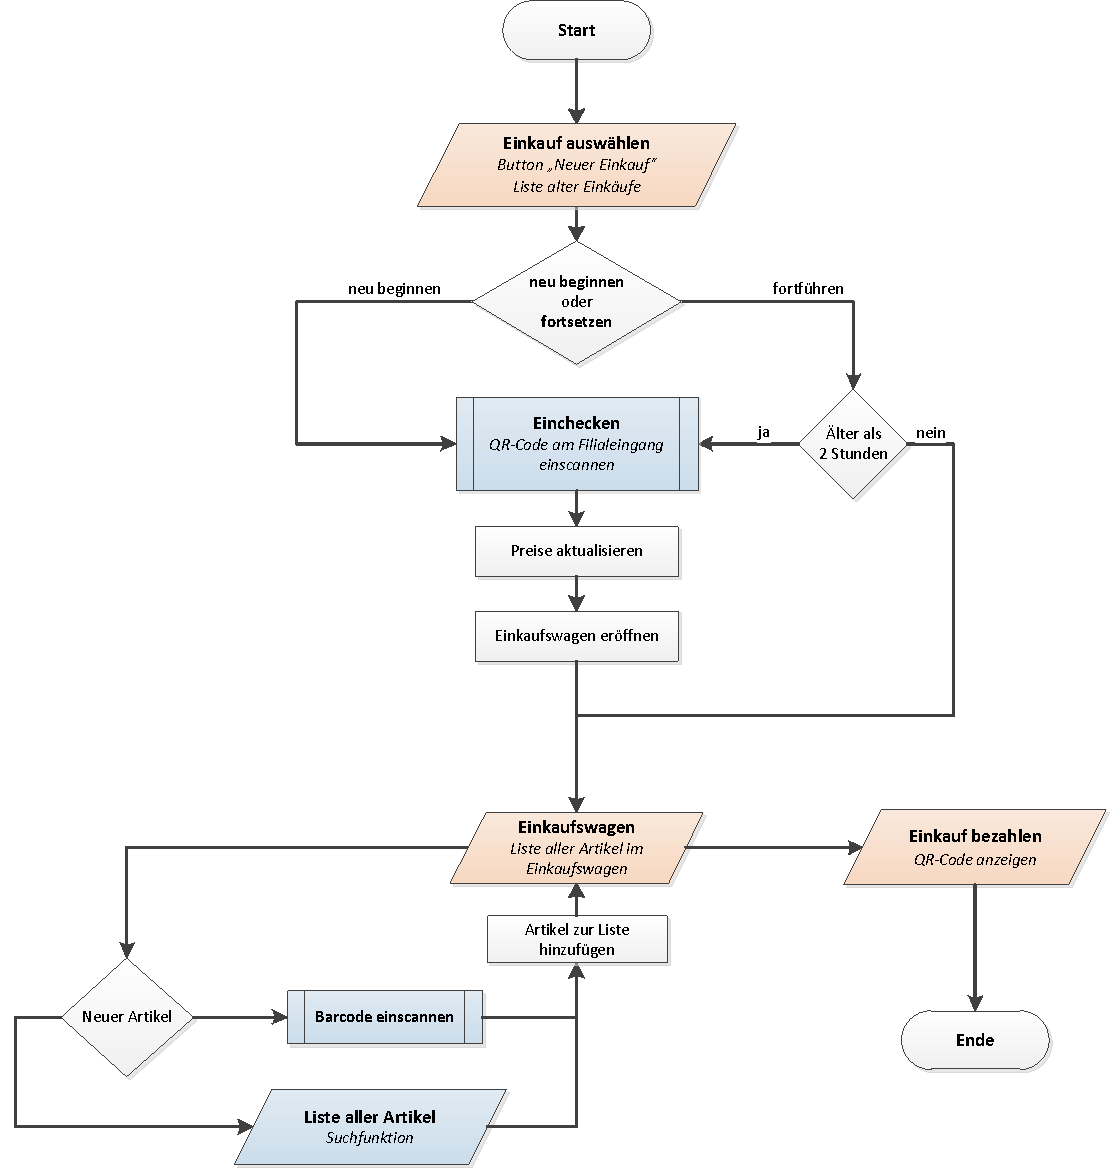
\includegraphics[width=\linewidth]{res/pap.pdf}
\caption{Programmablaufplan der SelfScanning-App}
\end{figure}

\subsection{Einkauf auswählen}
Im ersten Schritt soll der Kunde zunächst zwischen den zwei Möglichkeiten wählen, einen neuen Einkauf zu beginnen oder einen vorherigen fortzusetzen (vgl. oberstes grünes Trapez „Einkauf auswählen“ im PAP). Aufgrund der Anforderung, dass „alle Preise bis zum Zeitpunkt des Betretens der Filiale auf dem Smartphone verfügbar sein müssen“ [Referenz], wird vor jedem neuen Einkauf ein  Zwischenschritt eingeführt, der im Folgenden „Einchecken“ genannt wird.

Beim Einchecken handelt es sich um einen Prozess, bei dem der Kunde einen QR-Code im Eingangsbereich der Filiale einscannen muss. Hierbei lassen sich zusätzliche Informationen an das Smartphone übertragen, die für den Einkauf notwendig sind (bspw. Preisveränderungen, die erst kurz vor dem Einkauf entstanden sind). Eine detaillierte Beschreibung dieser Schnittstelle folgt im [Kapitel: Schnittstellendefinition – Smartphone->Kasse].

Der Nutzer hat darüber hinaus die Möglichkeit, einen bereits angefangenen Einkauf fortzuführen. Daran knüpft sich jedoch die Bedingung, dass das Erstellungsdatum des Einkaufs nicht mehr als 2 Stunden in der Vergangenheit liegt. Ansonsten ist eine Aktualität der Preise nicht mehr gewährleistet. In diesem Fall muss der Nutzer erneut einchecken. [Einkauf dann mit alten Artikeln fortsetzen? Gibt keine entsprechende Anforderung! Ggf. ergänzen.]

\subsection{Artikel hinzufügen}
Nachdem ein neuer Einkauf eröffnet bzw. ein bestehender fortgesetzt wurde, befindet sich der Kunde im „Einkaufswagen“-Dialog (vgl. grünes Trapez „Einkaufswagen“ in der Mitte des PAP). Hier lassen sich neue Artikel zum Einkaufswagen hinzufügen, bestehende editieren oder entfernen.

Das Hinzufügen erfolgt entweder per Einscannen des Barcodes auf einer Artikelverpackung oder per manueller Suche in einer Datenbank (falls keine Verpackung/Barcode vorhanden ist). Gesucht werden kann nach Artikelbezeichnung oder PLU-Nummer.

\subsection{Einkauf bezahlen}
Sobald sich alle Artikel im Einkaufswagen befinden, soll der Kunde seinen Einkauf an einer der herkömmlichen Kassen bezahlen können. Hierfür ist eine zweite Schnittstelle zum Informationsaustausch zwischen Smartphone und Kasse notwendig, die im [Kapitel: Schnittstellendefinition – Smartphone->Kasse] näher beschrieben ist.

\section{Sencha Touch und das MVC-Konzept}
Zur Strukturierung komplexer Anwendungen bietet Sencha Touch wie oben bereits erwähnt, ein Architekturkonzept, das auf dem MVC-Prinzip aufsetzt und dieses mit zusätzlichen Komponenten erweitert. Die SelfScanning-App soll mithilfe von Sencha Touch realisiert werden. Der in diesem Projekt beschriebene Entwurf basiert daher auch auf der von Sencha Touch verwendeten Architektur, die im Folgenden näher beschrieben wird.

\subsection{Das MVC-Konzept}
Zentraler Aspekt von MVC ist die strikte Trennung von Datenhaltung, Darstellung und Steuerung. Diese drei Bereiche werden im Folgenden Model, View und Controller genannt.

Durch die Aufteilung wird das System sehr leicht skalierbar und bleibt trotzdem flexibel. So können beispielsweise weitere Views unabhängig von Model und Controller hinzugefügt, bestehende Views entfernt oder ausgetauscht werden.

Das MVC-Konzept entspringt der Idee des sog. Beobachter-Musters. Diesem Muster zufolge unterscheidet man zwischen Objekten, die die Rolle eines Beobachters einnehmen und solchen, die beobachtet werden. [OO Programmierung, S. 512] Beobachtete Objekte kennen ihre Beobachter, sodass diese über Zustandsänderungen benachrichtig werden können. Die Beobachter wiederum können dann bei Bedarf den geänderten Zustand erfragen. Abbildung [OO Programmierung, S. 512] verdeutlicht dieses Konzept.

Um zu verstehen, wie dieses Muster nun Anwendung innerhalb des MVC-Konzepts findet, sollen zunächst die grundlegenden Begriffe Model, View und Controller geklärt werden.

\paragraph{Das Model} enthält fachlich strukturierte Informationen [Effekt. Software Arch., S. 247] und verwaltet einen konkreten Zustand. Außerdem liefert es Informationen zu seinem Zustand oder ändert diesen nach Aufforderung. [OO Programmierung, S. 516] 

\paragraph{Der View} dagegen ist ausschließlich für die Darstellung (Ausgabe) der Daten zuständig. Der entsprechende Input hierfür wird von den Models geliefert. Außerdem hat ein View die Zusatzaufgabe Benutzereingaben entgegenzunehmen und diese an den Controller weiterzuleiten.

\paragraph{Die Aufgabe des Controllers} war ursprünglich die Verarbeitung von Benutzerinteraktionen, um beispielsweise einen Mausklick einem konkreten Button zuzuordnen. Diese Aufgaben werden heutzutage allerdings von Modulen übernommen, die in Betriebssystemen, Browsern oder Basisbibliotheken integriert sind [OO Programmierung, S.515] Ein Controller im heutigen Sinne ist für die Ablaufsteuerung einer Anwendung und die Ausführung entsprechender Operationen zuständig. Typisches Beispiel hierfür wäre die Änderung der im Model enthaltenen Daten, nachdem der Benutzer ein Eingabeformular ausgefüllt und abgeschickt hat. Anschließend beauftragt der Controller

Das Beobachter-Muster findet innerhalb des MVC-Konzepts zweifache Anwendung:
\begin{itemize}
	\item View beobachtet Model\\
	Jeder View kann sich in die Beobachterliste eines Models eintragen. So kann das Model alle beobachtenden Views bei Aktualisierung der Daten benachrichtigen. Die Views wiederum aktualisieren dann bei Bedarf ihre Darstellung.
	\item Controller beobachtet View\\
	Außerdem kann ein Controller Views beobachten, um im Falle von Benutzereingaben benachrichtigt zu werden. Der Controller holt sich die Eingaben bei Bedarf und leitet weitere Schritte ein.
\end{itemize}

\subsection{Besonderheiten von Sencha Touch}

Sencha Touch bietet neben diesen drei Standardkomponenten diverse zusätzliche Komponenten an. Im Folgenden sollen lediglich die für das Projekt relevanten Bestandteile von Sencha Touch erklärt werden:

\paragraph{Der Store} beinhaltet Model-Instanzen eines bestimmten Typs. Er stellt Funktionen bereit, um die Sammlung an Model-Instanzen zu sortieren, zu gruppieren oder zu filtern. Außerdem können einzelne Model-Instanzen hinzugefügt, verändert oder entfernt werden.

\paragraph{Proxies }werden von Stores benutzt, um die Daten eines Models aus dem Speicher zu laden bzw. diese wieder in den Speicher zu schreiben. Bei dem Speichermedium muss es sich allerdings nicht immer um die lokale Festplatte handeln. Auch die Verbindung zu einer externen Datenbank oder einem Webservice wären denkbare Möglichkeiten.

\paragraph{Model-Assoziationen}
Zusätzlich zu den herkömmlichen Eigenschaften eines Models bietet Sencha Touch die Möglichkeit, einzelne Model-Typen miteinander in Beziehung zu versetzen. Dabei werden die drei Beziehungstypen „belongsTo“, „hasOne“ und „hasMany“ unterschieden. [Sencha Docs - Ext.data.association.Association] Anhand eines Besitzer-Auto-Motor Beispiels lassen sich die Beziehung wie folgt erklären
\begin{itemize}
	\item Jedes Auto gehört zu einem Besitzer (belongsTo)
	\item Ein Besitzer kann mehrere Autos besitzen (hasMany)
	\item Jedes Auto hat genau einen Motor (hasOne)
\end{itemize}
Eine Model-Instanz kennt seine in Beziehung stehenden Model-Instanzen. Sencha Touch stellt auf Basis dieser Tatsache zusätzliche Funktionen bereit, um Model-Assoziationen zu traversieren. Im Falle des obigen Beispiels lässt sich also mithilfe einer Besitzer-Instanz (aufgrund der hasmany-Beziehung) ein Store erzeugen, der alle Autos dieses Besitzers enthält – durch einen einzigen Funktionsaufruf.

\section{Anwendung der MVC-Architektur}
Die im vorherigen Kapitel beschriebenen Komponenten sollen nun auf den Entwurf der SelfScanning-App angewendet und näher beschrieben werden.

\subsection{Zu erstellende Views}
Aus dem in [Kapitel: Prinzipieller Programmablauf] abgebildeten Programmablaufplan lassen sich die folgenden drei Benutzerdialoge anhand der grün ausgefüllten Trapezen identifizieren: Einkauf auswählen, Einkaufswagen und Bezahlung. Diese drei Dialoge entsprechen jeweils einem separaten View. Zusätzlich soll ein weiterer View für die manuelle Suche von Artikeln erstellt werden. Die folgende Abbildung veranschaulicht die Reihenfolge und Bestandteile der einzelnen Views:

\begin{figure}[H]
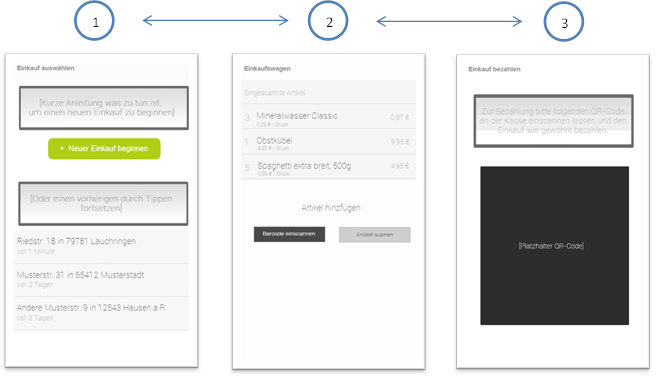
\includegraphics[width=\linewidth]{res/views.png}
\caption{Abfolge der drei Benutzerdialoge}
\end{figure}

\subsection{Models und zugehörige Assoziationen}
Anhand der fachlichen Anforderungen wurden die folgenden Models identifiziert, die in der [Abbildung: Models und Assoziationen] zu sehen sind.

\begin{figure}[H]
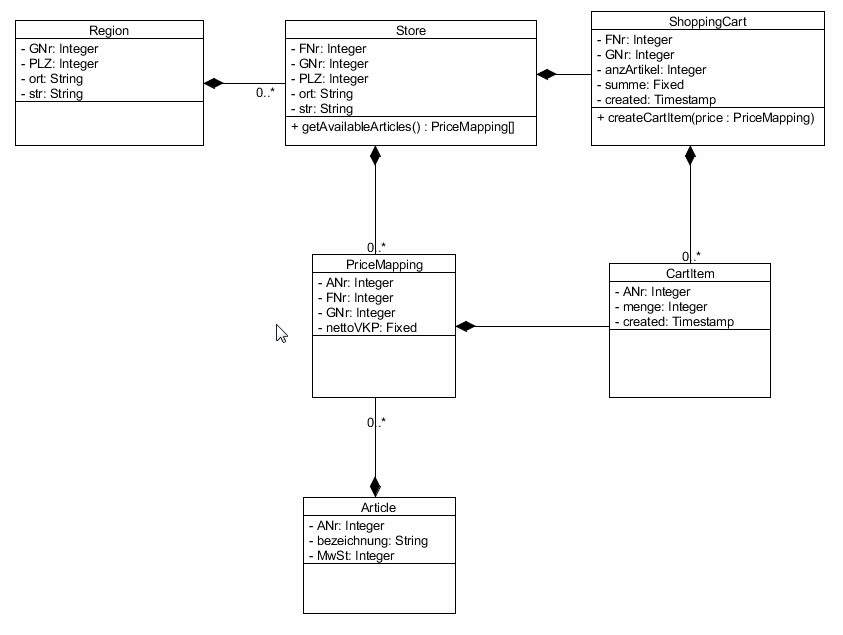
\includegraphics[width=\linewidth]{res/models.png}
\caption{Zu implementierende Models und zugehörige Assoziationen}
\end{figure}

An erster Stelle stehen die beiden Models „Region“ und „Store“, um Gesellschaften und Filialen abzubilden. Diese besitzen eine landes- bwz. regionalweit eindeutige Nummer („GNr“- bzw. „FNr“-Attribut). Da jede Filiale Teil einer Gesellschaft ist (Komposition), wird sie anhand ihrer Filialnummer in Kombination mit der zugehörigen Gesellschaftsnummer identifiziert.

Außerdem gibt es ein „Article“-Model, das eine eindeutige Artikelnummer („ANr“), sowie weitere Artikelinformationen enthält. Zu einem Article gehören beliebig viele „PriceMapping“-Models. Mit deren Hilfe kann ein Artikel einer Filiale zugeordnet werden, mit der Zusatzinformation zu welchem Verkaufspreis der Artikel in dieser Filiale angeboten wird. Andersrum formuliert besitzt ein Store beliebig viele PriceMappings, wodurch sich eine Liste aller in dieser Filiale verfügbaren Artikel inkl. der zugehörigen Verkaufspreise ergibt.

Letztlich bleibt noch das „ShoppingCart“-Model, das alle Artikel („CartItems“) enthält, die im Einkaufswagen liegen. Jeder Einkaufswagen ist genau einer Filiale zugeordnet. Jedes CartItem wiederum genau einem PriceMapping.

\subsection{Stores und Proxies}
Zu jedem Model wurde ein zugehöriger Store angelegt, der die von Sencha Touch bereitgestellten Standardfunktionen (siehe [Kapitel: Sencha Touch – Stores]) anbietet. 

Außerdem besitzt jedes Model einen eigenen Proxy, um die Daten in einer lokalen Datenbank abzuspeichern. Die Models Region, Store, PriceMapping und Article besitzen zusätzlich einen sog. „RemoteProxy“, der sich mit einer zentralen Datenbank im Internet verbinden und von dort aktuelle Informationen beziehen kann.

\subparagraph{Der Controller}
Die Anwendung soll lediglich einen einzigen Controller enthalten, der alle drei Views gleichzeitig beobachtet und auf entsprechende Ereignisse reagiert.

\begin{figure}[H]
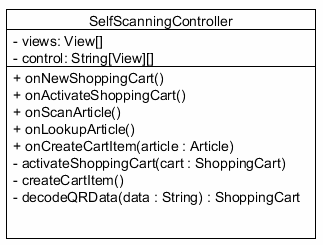
\includegraphics[scale=1]{res/controller.png}
\caption{Der zentrale Controller der Anwendung}
\end{figure}

\section{Einzelne Funktionen im Detail}
[HIER NOCH KAPITELEINLEITUNG SCHREIBEN]

\subsection{Einkauf eröffnen}
Das folgende Sequenzdiagramm zeigt den Prozess „Einkauf eröffnen“. Dieser wird angestoßen, wenn sich ein Nutzer im „Einkauf auswählen“-Dialog dafür entscheidet, einen neuen Einkauf zu beginnen. Hierfür ruft der Controller zunächst den Scanner auf, um den QR-Code im Eingangsbereich für den Check-In Prozess zu erfassen. Die darin enthaltenen Daten werden anschließend dekodiert und die entsprechenden Models (PriceMapping-Models) aktualisiert bzw. angelegt (ShoppingCart-Model). Das neu erstellte Model wird dann dem Einkaufswagen-View zugewiesen und angezeigt.

\begin{figure}[H]
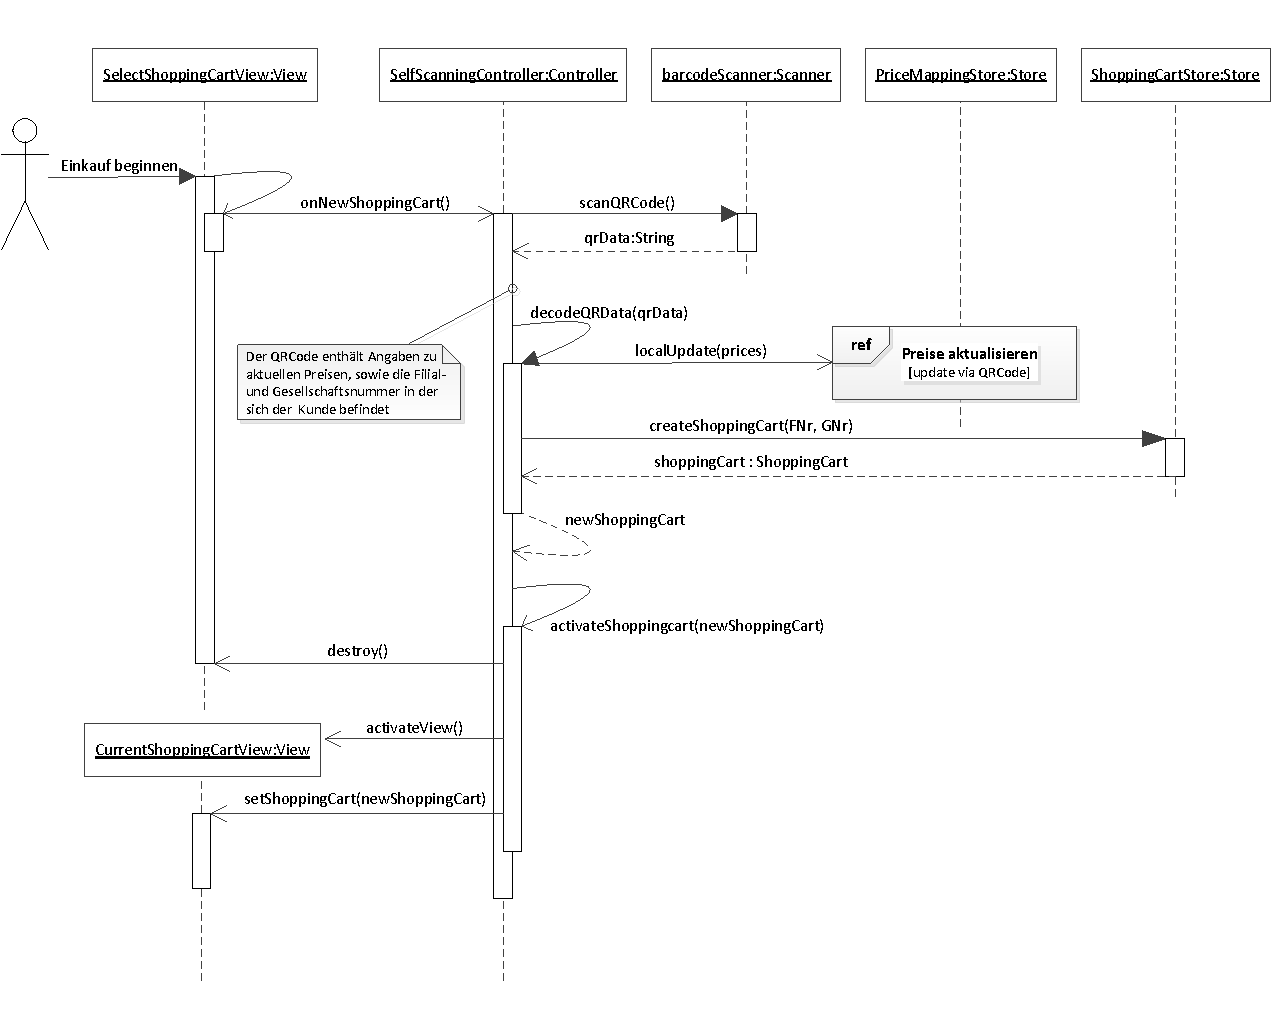
\includegraphics[width=\linewidth]{res/seq_einkauf-eroeffnen.pdf}
\caption{Der Prozess „Einkauf eröffnen“ als Sequenzdiagramm}
\end{figure}

\subsection{Artikel hinzufügen}
Um einen Artikel zu einem Einkaufswagen hinzuzufügen, bieten sich dem Nutzer zwei Möglichkeiten an: er scannt entweder den Barcode auf der Artikelverpackung oder sucht den passenden Artikel in einer Datenbank anhand Bezeichnung oder PLU-Nummer. Je nach Entscheidung werden die Methoden onScanArticle() bzw. onLookupArticle() ausgeführt, welche beide das passende Article-Model zurückliefern. Mit dessen Hilfe kann der Artikel dem aktuellen Einkaufswagen hinzugefügt und angezeigt werden.

\begin{figure}[H]
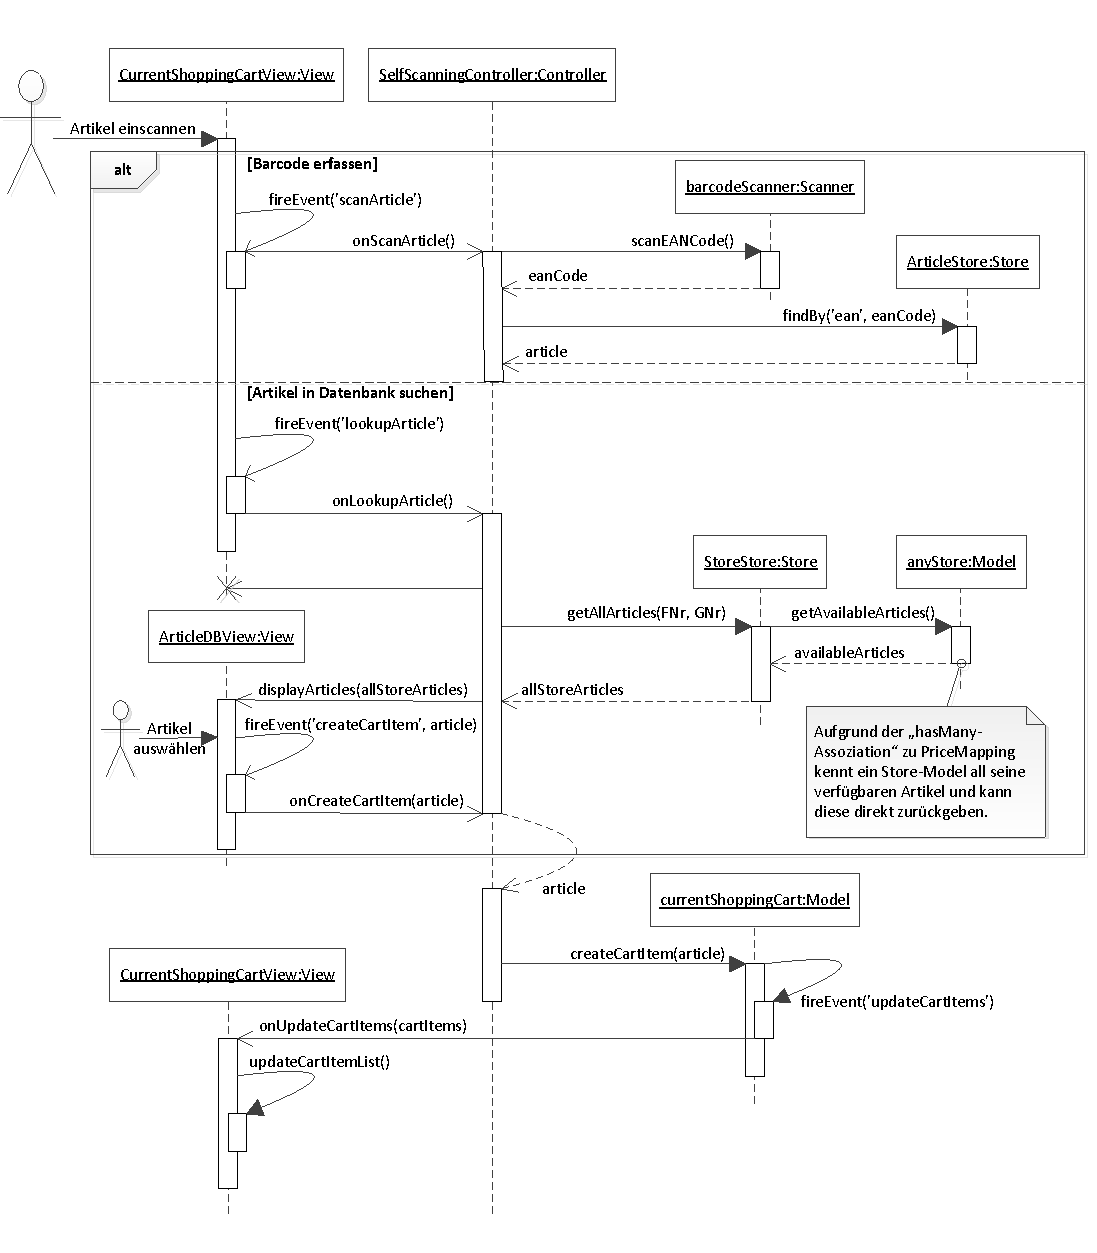
\includegraphics[width=\linewidth]{res/seq_artikel-hinzufuegen.pdf}
\caption{Der Prozess „Artikel hinzufügen“ als Sequenzdiagramm}
\end{figure}

\subsection{Preise updaten}
Preise lassen sich entweder anhand des QR-Codes beim Check-In aktualisieren oder nach Anstoßen der remoteUpdate()-Funktion, um ein Update über das Internet durchzuführen. Letzteres erfolgt über den PriceMappingProxy, der von einer zentralen Datenbank seine Daten bezieht.

\begin{figure}[H]
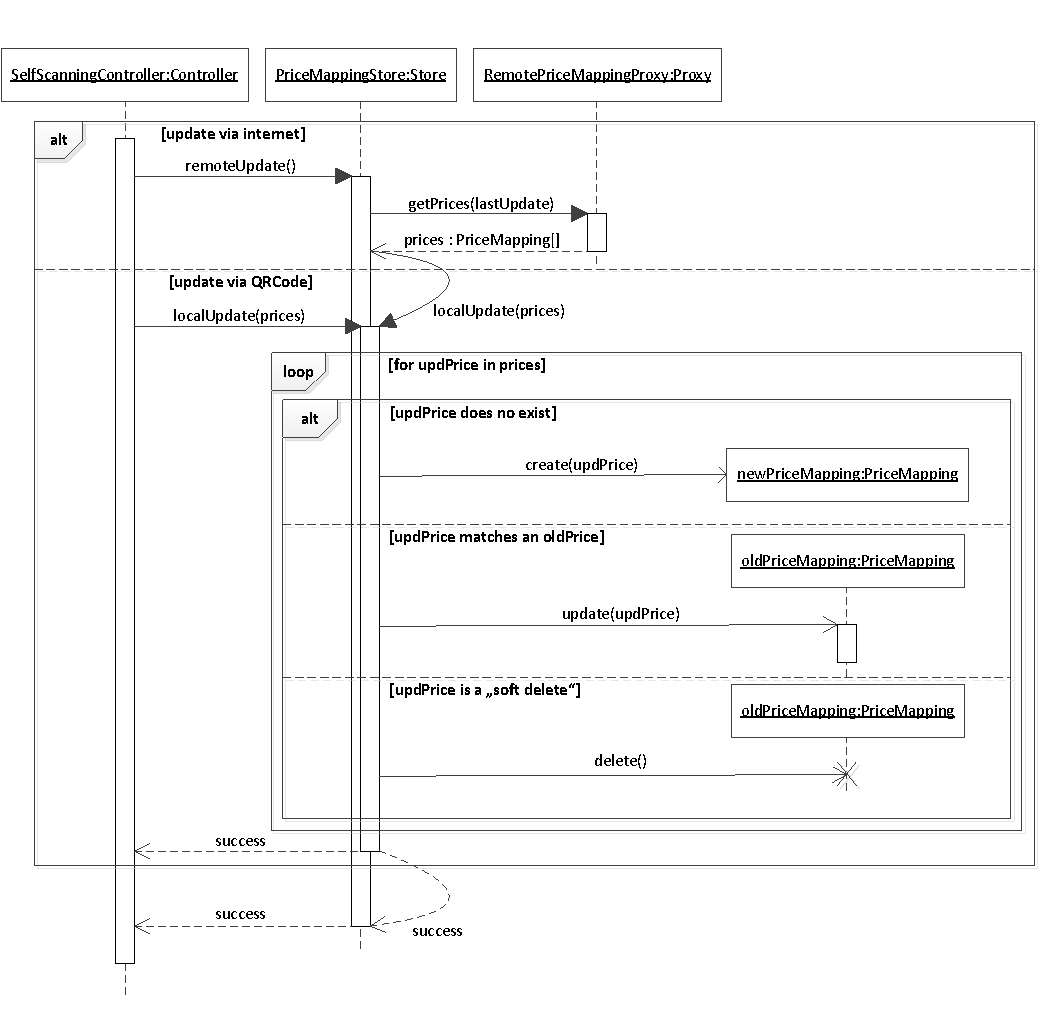
\includegraphics[width=\linewidth]{res/seq_preise-updaten.pdf}
\caption{Der Prozess „Preise updaten“ als Sequenzdiagramm}
\end{figure}

\section{Schnittstellenbeschreibungen}
[HIER NOCH KAPITELEINLEITUNG SCHREIBEN]

\subsection{Kasse zu Smartphone: Übertragung lokaler Preisänderungen}
Um dem Kunden auch dann aktuelle Preisinformationen zu bieten, wenn sein Smartphone nicht mit dem mobilen Internet verbunden ist, werden bei jedem Check-In die lokalen Preisveränderungen (LPVs) der Filiale an das Smartphone übertragen.

Hierfür muss der Kunde vor jedem Einkauf einen QR-Code im Eingangsbereich der Filiale einscannen. Dieser enthält Angaben zu seinem Standort (die Filiale in der er sich aufhält) und alle aktuell gültigen Preisveränderungen dieser Filiale. Die kodierten Informationen lassen sich als konkatenierten String darstellen, dessen einzelnen Bestandteile in der folgenden Tabelle zunächst aufgezählt und anschließend näher erläutert werden.

\begin{table}[H]
  \begin{center}\small\renewcommand{\arraystretch}{1.4}\sffamily % kleinere, serifenlose Schrift & größere Zeilen
  \begin{tabulary}{\textwidth}{ccl}
    Pos. & Länge & Beschreibung\\ \hline
    1 & 3 & Gesellschaftsnummer\\ 
    2 & 3 & Filialnummer\\
    3 & var & Filialpreise\\ 
    4 & 5 & Separator\\ 
    5 & var & Gesellschaftspreise\\
    6 & 5 & Separator\\
    7 & var & Landespreise
   \end{tabulary}      
 \caption{Bestandteile des QR-Codes im Filialeingang}
 \label{tab:uebersicht-vergleich}
 \end{center} 
\end{table}

\begin{seToplist}{1. }
\item[1. ]\textbf{Gesellschaftsnummer} (3 stellig)\label{interface-gnr}\\
	Nummer der Regionalgesellschaft\\
	\textit{Beispiel}: 012 für Gesellschaft 12 (Donaueschingen)
	
\item[2. ]\textbf{Filialnummer} (3 stellig)\\
	Nummer der Filiale\label{interface-fnr}\\
	\textit{Beispiel}: 053 für Filiale 53 (Riedstr. 18 in Lauchringen)
\item[3. ]\textbf{Filialpreise} (variable Länge)\label{interface-fpreise}\\
	Das Filialpreisfeld ist wiederum ein zusammenhängender String aus einzelnen Artikelnummern und Preisen.	Die ersten 5 Stellen enthalten die Artikelnummer (im Falle von kürzeren Artikelnummern werden die Stellen von links mit Nullen aufgefüllt). Die folgenden und auch letzten 5 Stellen enthalten den Preis ohne Dezimaltrennzeichen, wobei die letzten beiden Ziffern als 1/10 und 1/100 Stellen interpretiert werden.
	\begin{seToplist}{Beispiel: }
		\item[\textit{Beispiel}:] 0123400595313379950 für 
		\begin{itemize}
		\item[-] den Artikel 1234 zu einem Preis von 5,95 \euro
		\item[-] den Artikel 31337 zu einem Preis von 99,50 \euro
		\end{itemize}
	\end{seToplist}
	\textit{Wichtige Hinweise}
	\begin{itemize}
	\item[-] Die Artikelnummer 00000 darf nicht vergeben werden! Die Zeichenfolge ist für den Separator (siehe unten) reserviert.
	\item[-] Ein Preis der als 00000 kodiert ist, ist ein sogenannter „soft delete“. D.h. diese Preisveränderung ist nicht länger gültig und muss (falls vorhanden) in der Datenbank des Smartphones entfernt werden. 
	\end{itemize}
	
\item[4. ]\textbf{Separator} (5 stellig)\\
	Das Separatorfeld ist eine reservierte Zeichenkette aus fünf Nullen („00000“). Es dient dazu, die Filialpreise von den Gesellschaftspreisen zu trennen.
	
	\textit{Wichtiger Hinweis}
		\begin{itemize}
		\item[-] Dieses Feld wird nur dann angehängt, wenn Gesellschaftspreise enthalten sind.
		\end{itemize}
		
\item[5. ]\textbf{Gesellschaftspreise} (variable Länge, optional)\\
	Pendant zu den Filialpreisen. Siehe \textit{3. Filialpreise} für weitere Details.
	
\item[6. ]\textbf{Separator} (5 stellig)\\
	Siehe \textit{4. Separator}.
	
	\textit{Wichtiger Hinweis}
			\begin{itemize}
			\item[-] Dieses Feld wird nur dann angehängt, wenn Landespreise enthalten sind.
			\end{itemize}
			
\item[7. ]\textbf{Landespreise} (variable Länge, optional)\\
	Pendant zu Filial- und Gesellschaftspreisen. Siehe \textit{3. Filialpreise} für weitere Details.
\end{seToplist}

Durch den nachfolgenden QR-Code wird ein Beispiel gegeben, das alle oben beschriebenen Informationen enthält. Sein Inhalt kann mit einer gewöhnlichen QRCode-Reader App nachgeprüft werden:

\begin{figure}[H]

\includegraphics[scale=1]{res/qr_eingang}
\caption{Beispielhafter QR-Code mit lokalen Preisveränderungen}
\end{figure}

\texttt{\textcolor{red}{012}\textcolor{orange}{053}\textcolor{blue}{01111}\textcolor{brown}{00000}\textcolor{cyan}{01235}\textcolor{brown}{00050}\textcolor{cyan}{05555}\textcolor{brown}{00000}\textcolor{cyan}{06666}\textcolor{brown}{00000}\textcolor{cyan}{09999}\textcolor{brown}{00000}\textcolor{violet}{00000}\\
\textcolor{cyan}{05555}\textcolor{brown}{00500}\textcolor{cyan}{06666}\textcolor{brown}{00019}\textcolor{cyan}{09999}\textcolor{brown}{00000}\textcolor{violet}{00000}\textcolor{cyan}{01111}\textcolor{brown}{00995}\textcolor{cyan}{01234}\textcolor{brown}{01900}\textcolor{cyan}{01235}\\
\textcolor{brown}{00029}\textcolor{cyan}{05555}\textcolor{brown}{01250}\textcolor{cyan}{06666}\textcolor{brown}{00600}\textcolor{cyan}{09999}\textcolor{brown}{00000}\textcolor{cyan}{12345}\textcolor{brown}{00556}}

\subsection{Smartphone zu Kasse: Übertragung der eingescannten Artikel}
Nachdem der Kunde alle Waren eingescannt hat, muss der virtuelle Einkaufswagen an das Kassensystem übertragen werden. Hierfür wird auf dem Display des Smartphones ein QR-Code angezeigt, der die Artikelnummern und zugehörigen Mengen aller eingescannten Waren enthält.

Der Inhalt des QR-Codes lässt sich als konkatenierten String darstellen. Seine einzelnen Bestandteile werden im Folgenden näher beschrieben.

\begin{table}[H]
  \begin{center}\small\renewcommand{\arraystretch}{1.4}\sffamily % kleinere, serifenlose Schrift & größere Zeilen
  \begin{tabulary}{\textwidth}{ccl}
    Pos. & Länge & Beschreibung\\ \hline
    1 & 3 & Gesellschaftsnummer\\ 
    2 & 3 & Filialnummer\\
    3 & 3 & Anzahl Artikelpositionen\\ 
    4 & var & Artikeldetails\\ 
    5 & 2 & Anzahl Pfandbons\\
    6 & ? & Pfandbons\\
    7 & 6 & Summe
   \end{tabulary}      
 \caption{Bestandteile des QR-Codes auf dem Smartphone}
 \label{tab:uebersicht-vergleich}
 \end{center} 
\end{table}

\begin{seToplist}{1. }
\item[1. ]\textbf{Gesellschaftsnummer} (3 stellig)\\
	Analog zu \textit{1. Gesellschaftsnummer} in \ref{interface-gnr}.
	
\item[2. ]\textbf{Filialnummer} (3 stellig)\\
	Analog zu \textit{2. Filialnummer} in \ref{interface-fnr}.
	
\item[3. ]\textbf{Anzahl Artikelpositionen} (3 stellig)\\
	Anzahl aller Artikelpositionen (nicht die Gesamtmenge aller Artikel) im Einkaufswagen, zur Berechnung des hierauf folgenden Feldes (Artikelinformationen).
	
		\textit{Wichtiger Hinweis}
			\begin{itemize}
			\item[-] verknüpfte Artikel (z.B. Pfand) sollen hier nicht enthalten sein, da sie auch nicht Bestandteil des nächsten Feldes sind.
			\end{itemize}
	
\item[4. ]\textbf{Artikeldetails} (variabel)\\
	Dieses Feld beinhaltet jeweils die Artikelnummer (5 stellig) mit zugehöriger Menge (2 stellig) jedes eingescannten Produkts. Artikelnr. und Menge werden gegebenenfalls von links mit Nullen aufgefüllt.
	
	\begin{seToplist}{Beispiel: }
			\item[\textit{Beispiel}:] 01234033133701 für 
			\begin{itemize}
			\item[-] 3 Stück von Artikel 1234
			\item[-] 1 Stück von Artikel 31337
			\end{itemize}
		\end{seToplist}
		\textit{Wichtiger Hinweis}
		\begin{itemize}
		\item[-] Verknüpfte Artikel (Pfand) sollen hier nicht enthalten sein. Diese werden von der Kasse erneut dem Kassenbon hinzugefügt.
		\end{itemize}
		
\item[5. ]\textbf{Menge der Pfandbons} (2 stellig)\\
	Menge der im Einkaufswagen enthaltenen Pfandbons. Wird ggf. von links mit Nullen aufgefüllt.
	
\item[6. ]\textbf{Pfandbons} (variabel)\\
	TODO
			
\item[7. ]\textbf{Gesamtsumme} (6 stellig)\\
	An der Kasse zu zahlender Betrag. Die Summe besteht aus 6 Zeichen, ohne Dezimaltrennzeichen. Die letzten beiden Ziffern werden als $\frac{1}{10}$ bzw. $\frac{1}{100}$ Stelle interpretiert. 
\end{seToplist}


% Anhang der Arbeit
% 
%
\seAppendix{}
\chapter{Einige wichtige \LaTeX{}-Kommandos}

%
%  Erzeugung eines Glossars
%
% Achtung: Das Glossar wird nur ausgegeben, wenn mindestens ein Eintrag in der Arbeit 
%                definiert wurde
%
%
\newpage
\sePrintGlossary{}


%
% Literaturverzeichnisses
%
%\newpage
\sePrintBibliography{}

%  Erzeugung von Eintr\"agen im Literaturverzeichnis
%
%  Achtung: in einer Projektarbeit darf da \nocite-Kommando nicht verwendet werden,
%                 da es einen Eintrag im Literaturverzeichnis erzeugt, ohne dass eine 
%                 entsprechende Literaturreferenz im Text der Arbeit angegeben wird
%
%
%



\nocite{DHBW:SG}
\nocite{KM:KS}
\nocite{Dud06}
\nocite{Dud09}
\nocite{Bri:WA}
\nocite{RP:WA}
\nocite{Sch:WAS}
\nocite{BSS:WA}
\nocite{Kor:WA}
\nocite{MK:GWA}
\nocite{ADG:WA}
\nocite{The:WA}
\nocite{BA:WA}
\nocite{Dij:CRT}
\nocite{BC:Cur}
\nocite{Par:ECP}
\nocite{Bro:SBE}
\nocite{GI:ADI}
\nocite{GI:AZI}
\nocite{Den:CD}
\nocite{LMS:Icb}
\nocite{Fre:SIF}




%
% Festlegung des grundlegenden Formatierungsstils des Literaturverzeichnis
%
\bibliographystyle{jurabib}

% Eigentliche Ausgabe der in der Arbeit verwendeten Quellen
%
%
% Angabe der bib-Dateien, in denen die Quellen beschrieben sind;
% die Angabe geht davon aus, dass eine wa.bib-Datei in demselben 
% Verzeichnis liegt, wie se-ba-vorlage.tex
%

% 2012-02-06
%
% Umbenennung von Literatur- in Quellenverzeichnis
% 
%\renewcommand*{\bibname}{Quellenverzeichnis}
\seBibliography{wa}


%
% Erzeugung der ehrenw\"ortlichen Erkl\"arung
%
% Der optionale Parameter kann verwendet werden, um f\"ur das Thema der Arbeit eine 
% andere Formatierung vorzunehmen; das sollte in der Regel nicht erforderlich sein;
% ausserdem besteht die Gefahr inkonsistenter Titel auf dem Titelblatt und in der 
% ehrenw\"ortlichen Erkl\"arung
%
%\seEhrenwoertlicheErklaerung{} % dieses Kommando sollte standardm\"assig verwendet werden
\seEhrenwoertlicheErklaerung[\seThemaWaArbeit{}]


\end{document}